\chapter{State of the art}
\label{Chap2}
\section{Selective laser melting technology}
Selective laser melting (SLM) - also referred to as direct metal laser sintering (DMLS) - is an additive manufacturing  (AM) technique making use of a high power-density laser that locally melts powder materials.%Layers are progressively piled up, in order to create a 3D part. 
 When a layer of powder has been melted, a new layer is spread on top of the previous one, and is in turn melted, in order to progressively build a 3D object. The technique is illustrated on figure \ref{fig:SLM} \parencite{LEITZ2017331}. The materials used include mostly metals but also ceramics and composites. Parts to build must first be drawn in a computer-aided design (CAD) software and broken down in 2D slices, each one corresponding to a powder layer. During the process, the oxygen pressure $p_{O_2}$ must be kept low to prevent the oxidation of the metal. A shielding gas - such as argon - is thus used to fill the build chamber at all time, while $p_{O2}$ is monitored.   \\

\begin{figure}[th]
\centering
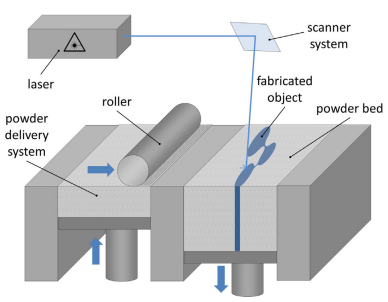
\includegraphics[scale=0.7]{Images/SLM}
\decoRule
\caption[Selective laser melting technology principle]{Selective laser melting technology principle (from Leitz et al., 2016).}
\label{fig:SLM}
\end{figure}

LSM is still a young technology. Its popularity only increased significantly over the last decade, as depicted by figures \ref{fig:Evol} (a) and (b). Works concerning AlSi10Mg began to emerge noticeably in 2014. The technique usage spread rapidly in many sectors: biomedical, heat exchangers, aerospace and automotive - to name just a few \parencite{Yap}. This is due to the numerous appeals of SLM compared to the other technologies, including:\\

\begin{itemize}
\item Geometrical flexibility: parts can be designed with thin walls or even with hidden cavities and/or channels. This offers promising prospects regarding light-weight potentials for parts solicited mechanically \parencite{Lippert};
\item Increased reliability of the parts \parencite{Haase};
\item Reduced equipment costs \parencite{Hoeges};
\item Better operational efficiency: the fabrication is quick and easy which reduces time-to-market as well as assembly times and capital tied up in stocks \parencite{Hoeges};
\item Individual production facilitation \parencite{Haase};
\item Reduced material waste and better energy usage: the process is  environmentally friendly as a whole \parencite{Haase}.
\end{itemize}

\begin{figure}[th]
\centering
\noindent\makebox[\textwidth]{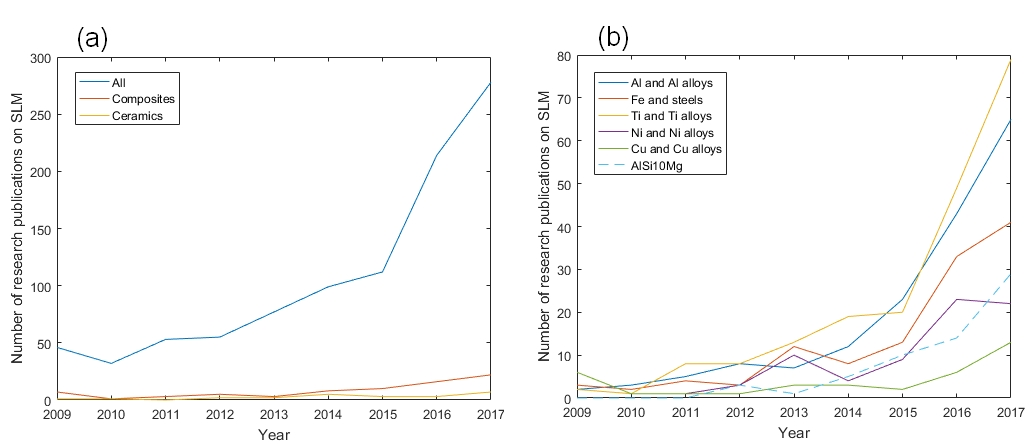
\includegraphics[scale=0.55]{Images/Evol}}
\decoRule

\caption[(a)Research publications on SLM of ceramics, composites and all materials types combined. (b)Research publications on SLM of different metallic materials]{(a)Research publications on SLM of ceramics, composites and all materials types combined. (b)Research publications on SLM of different metallic materials. Data are derived from the research publications on SLM, LaserCusing and DMLS existing on ScienceDirect website.}
\label{fig:Evol}
\end{figure}

The properties of parts produced trough SLM stem from the coupled effects of a great deal of parameters (see figure \ref{fig:param} ) \parencite{Aboulkair140820}.  %Les caractérisitiques des pièces produites grâce à la fusion laser sélective (SLM) sont le fruit de l'action simultanée et couplée d'un grand nombres de paramètres (see figure \ref{fig:param} ) \parencite{Aboulkair140820}.
Results are very sensitive to their variations. The process parameters must thus be monitored thoroughly. This complicates the search for their optimisation, still not fully resolved for aluminium alloys.\\%.Les résultats sont très sensibles à leurs variations et il est donc nécessaire de les contrôler méticuleusement. Pour ces raisons, il n'est pas simple d'étudier leurs impacts.\\
\begin{figure}[th]
\centering
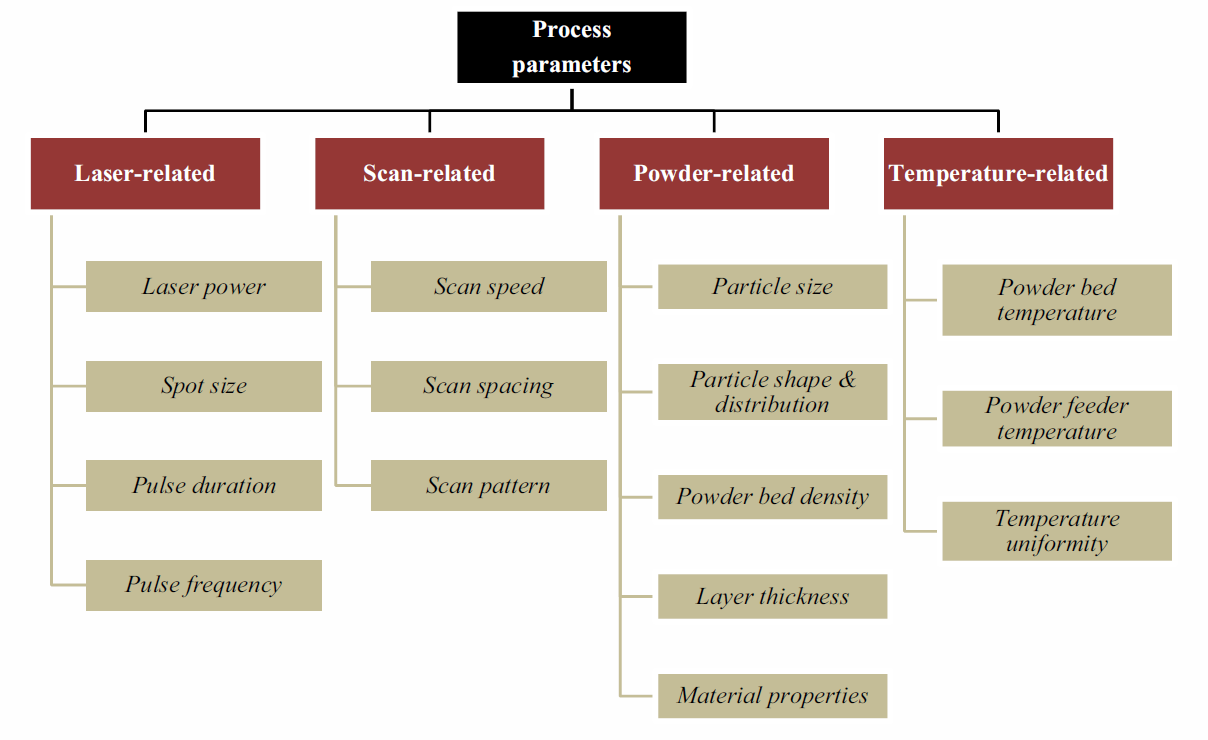
\includegraphics[scale=0.37]{Images/Param}
\decoRule

\caption[Parameters involved in SLM]{Parameters involved in SLM (from Aboulkhair et al., 2014).}
\label{fig:param}
\end{figure}

In recent years, works aiming at facing this challenge multiplied. The minimisation of the porosity is at the center of attention. It is indeed closely related to the quality of the mechanical properties. As porosity contributes to lowering the load-bearing surface, it reduces the apparent material strength. It was also observed to have a critical influence on the fatigue life of the produced parts. Their lifetime is especially diminished if the values of pores amount and size go beyond a certain threshold \parencite{Brandl121509}. Studies investigating the effects of various parameters on the AlSi10Mg fabrication trough SLM abound in the literature.\\

\section{AlSi10Mg alloy}
\textcolor{red}{Parler de l'AlSi10Mg; quel est l'interet de travailler avec? Difficultés? (reflectivité etc).. Qu'est ce qui existe en coulé, forgé etc}\\
\textcolor{red}{Microstructure homogène, diagramme de phase}\\

Kempen dans "PROCESS OPTIMIZATION AND MICROSTRUCTURAL ANALYSIS FOR SELECTIVE LASER
MELTING OF AlSi10Mg ":

AlSi10Mg is a typical casting alloy which is, due to its high strength/density ratio and thermal
properties, highly demanded in aerospace and automotive industries [1]. The alloy combination of aluminium,
silicon and magnesium results in a significant increase in strength and hardness which might even reach 300
MPa and 100 HBS, respectively, by applying a proper heat treatment [2]

Aluminium as a lightweight material is very attractive for the production of parts that require good
mechanical properties in combination with a low weight. The main focus lies on Al-Si alloys, since they are
casting alloys that are also suitable for welding. AlSi10Mg, which can be hardened by applying a specific heat
treatment, is relatively easy to process by laser applications due to the small difference between liquidus and
solidus temperature compared to high strength aluminium-alloys [2]. The AlSi10Mg alloy is frequently used in
aerospace, automotive, chemical and food industry. Its composition according to ISO 3522 can be found in
Table 1 [4]. Alloying the magnesium to the Al-Si alloy enables precipitation of Mg2Si which will strengthen the
matrix without compromising the other mechanical properties to a significant extent.
Table 1.Chemical composition of AlSi10Mg [4]
Alloying
element
Al Si Cu Mn Mg Zn Fe
wt % rest 9-11 < 0.1 0.05 0.45-0.6 0.05 < 0.55

\section{Fabrication process parameters}
\label{pp}
Let us now investigate the influence of the parameters on the properties of AlSi10Mg parts manufactured with SLM. The analysis of the paired impacts of the laser power P and scan speed $v_s$ provides a first insight. As depicted by figures \ref{fig:Pvs} and \ref{fig:Pvs2}, low P and high $v_s$ lead to an insufficient energy input to melt the powder and re-melt the substrate, which causes the formation of droplets \parencite{Kempen110817} . The opposite leads to good penetration but also to distortions and irregularities.   A trend to use both high P and $v_s$ rose in accordance with these findings. Doing so has the advantage to increase productivity. However, it also has multiple downsides including a decrease of the surface quality due to balling, excessive spatter, and an augmented gas induced porosity \parencite{Mertens170406}. Therefore, a trade-off must be found. \\

A popular approach is to regroup multiple operating parameters into one, the volumetric energy density $E_d$. It is estimated trough the following formula: 
$$E_d=\frac{P}{v_s h t} $$
where t is the layer thickness and h is the hatch space. As a rule of thumb, $E_d$ should be chosen in the range between 60 and 75 [$\frac{J}{mm^3}$] \parencite{Read150417}. However, the criterion is insufficient and others phenomena, such as melt pools overlapping, should be considered \parencite{Tang170309}. Very few studies were carried out to optimize h and t independently. Their values lie generally respectively in the intervals [50 ; 200] [$\mu m$] and [20 ; 60] [$\mu m$] \parencite{aboulkhair2016,Brandl121509,Kempen110817,Mertens170406}. It was observed that for t = 30 [$\mu m$], an optimal set of parameters values in terms of density is P = 200 [W], $v_s=1400 [\frac{mm}{s}]$ and h = 105 [$\mu m$] \parencite{Kempen110817}. The apparent relative density $\rho_{a,rel}$ was then above 99.5 [\%].\\

\begin{figure}[th]
\centering
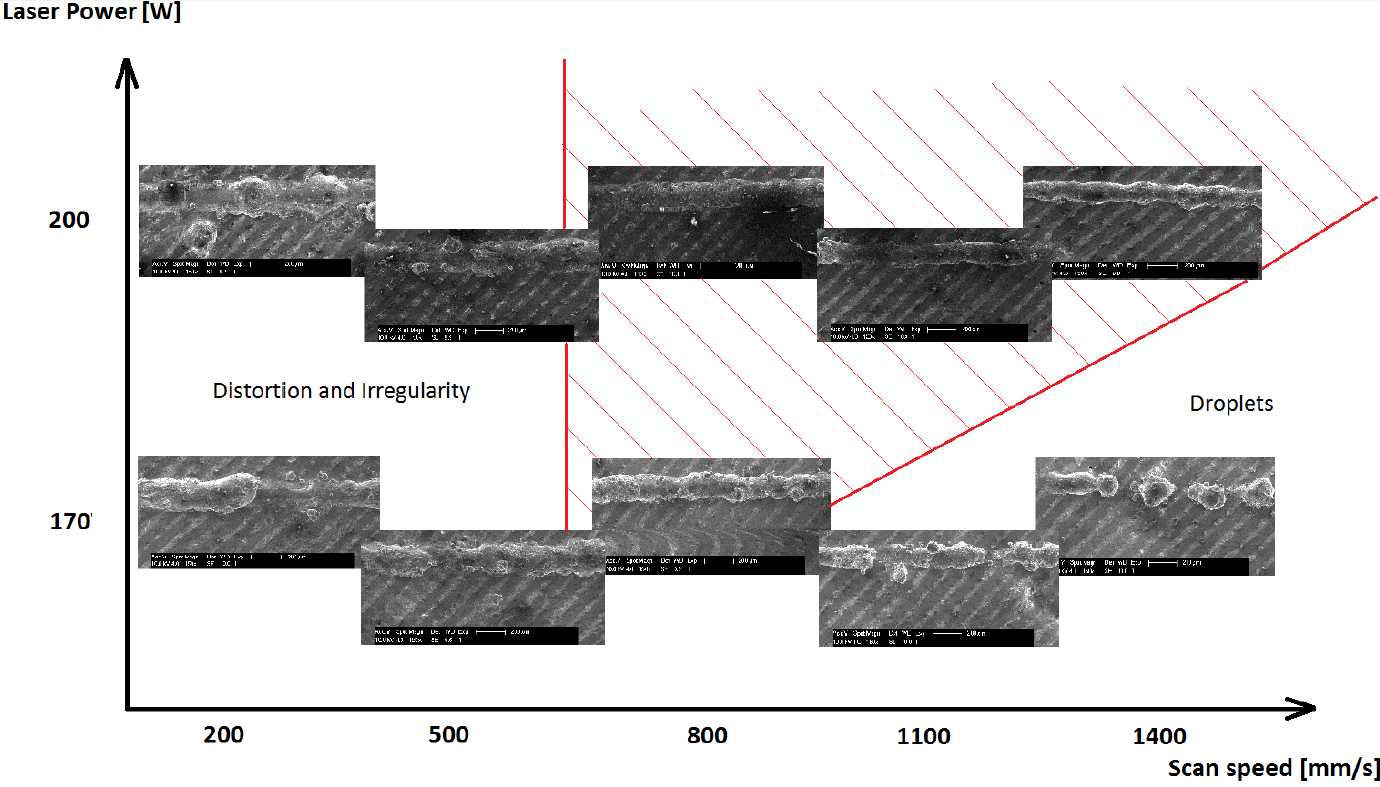
\includegraphics[scale=0.32]{Images/Pvs}
\decoRule
\caption[Process window for SLM of AlSi10Mg, based on the top view of single track scans]{Process window for SLM of AlSi10Mg, based on the top view of single track scans (from Kempen et al., 2011).}
\label{fig:Pvs}
\end{figure}

\begin{figure}[th]
\centering
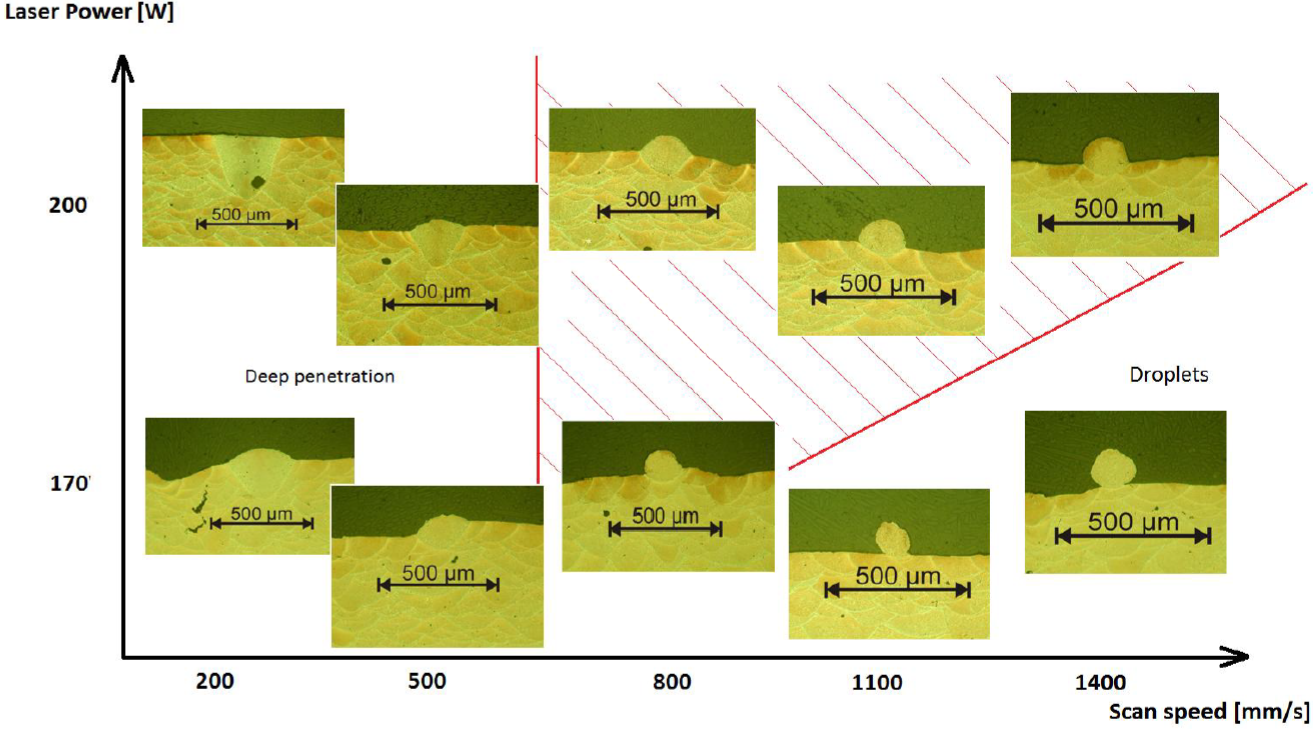
\includegraphics[scale=0.32]{Images/Pvs2}
\decoRule
\caption[Process window for SLM of AlSi10Mg, based on the front view of single track scans]{Process window for SLM of AlSi10Mg, based on the front view of single track scans (from Kempen et al., 2011).}
\label{fig:Pvs2}
\end{figure}

The other process parameters will be covered for the sake of completeness. Let us first look into the particle-related parameters. The particle size $D_a$ of the powder should be as small as possible to ensure a good flowability and allow for thin layers \parencite{Kempen110817}. Typical values for mean particle size stretch from 15 to 50 [$\mu m$] but are more often at around 30 [$\mu m$] \parencite{Brandl121509,Kempen110817,MOWER2016198,UZAN2017229}. The size distribution is more delicate to outline. On one hand, wider distributions often generate better bed density, parts with higher density and better surface finish. On the other hand, narrower ones usually provide better flowability and parts with better strength and hardness \parencite{Liu1101}. In most cases, a middle ground between the two should be sought. In SLM applications, powder is often successively recycled multiple times. This leads to their progressive contamination with moisture, which causes an increase of hydrogen porosity in the produced parts \parencite{Weingarten151102}. The problem can be overcome by drying the powder or using fresh one. Unfortunately - in the case of aluminium alloys - no findings were made regarding the prediction of a threshold at which one should take action \parencite{aboulkhair2017}.    \\

The choice of scan pattern has great importance. There exist a few different strategies. The common ones use unidirectional, bidirectional or islands patterns (see figure \ref{fig:Strat}). The scan direction(s) should always be rotated between successive layers to favorise isotropy, especially in the unidirectional case since it causes height variations along a layer \parencite{aboulkhair2016}. The islands pattern is based on a decomposition in small domains with short scanning tracks. Two usual strategies can be distinguished among this group: the chessboard and the hexagonal one. A study proved the superiority of an island pattern over a bidirectional one in terms of both ultimate tensile stress $\sigma_u$ and strain at fracture $\epsilon_f$ for a 316L stainless steel-Inconel 718 material \parencite{Zhou15}. It was also shown that it was possible to fabricate pure titanium samples without cracks using an island pattern, and not with a bidirectional one \parencite{Li17}. This is seemingly due to the greater accumulation of internal stresses and to the weaker interlayer bounding in the second case. \\

\begin{figure}[h!]
\centering
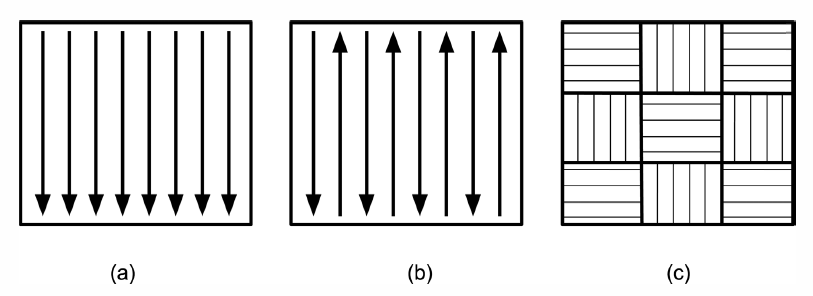
\includegraphics[scale=0.6]{Images/Strat}
\decoRule
\caption[Schematic representation of scanning strategies commonly used in LSM (a) unidirectional long scan track; (b) bi-directional long scan track, and (c) islands]{Schematic representation of scanning strategies commonly used in LSM (a) unidirectional long scan track; (b) bi-directional long scan track, and (c) islands (from Mertens et al., 2017).}
\label{fig:Strat}
\end{figure}

Furthermore, dual scanning strategies were proven to be effective. For example, a pre-scan with low $E_d$ can flatten the powder bed before it is consolidated, which leads to a reduction of porosity \parencite{Mertens170406}. It was also shown that scanning the contour of the part being built at lower $E_d$ can better the surface roughness for AlSi12Mg \parencite{PRASHANTH170205}. One should note too that the final properties of the fabricated part can strongly depend on the building direction (see figure \ref{fig:Build}) \parencite{DELROISSE201732}. Further properties comparison is provided in section \ref{MMABMP}

\begin{figure}[th]
\centering
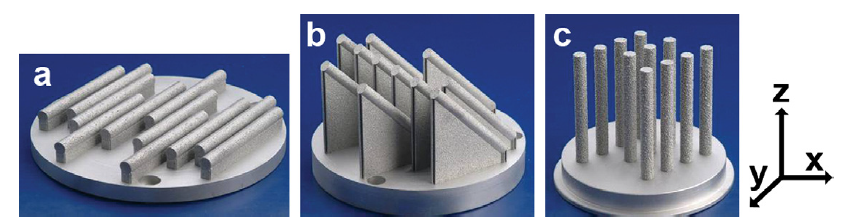
\includegraphics[scale=0.58]{Images/Build}
\decoRule
\caption[Samples (static tensile) built in different directions: (a) $0^\circ$, (b) $45^\circ$, and (c) $90^\circ$]{Samples (static tensile) built in different directions: (a) $0^\circ$, (b) $45^\circ$, and (c) $90^\circ$ (from Brandl et al., 2012).}
\label{fig:Build}
\end{figure}


Other laser-related parameters - the spot size and the pulse properties - can also influence the process. Only the laser spot size at the 99\% contour $\phi_{99\%}$ is frequently cited in literature. Its value lies between 20 and 200 [$\mu m$] \parencite{Brandl121509,Kempen110817,MOWER2016198}. At this moment, no optimisation study was carried out about this variable. One should expect the optimal value for P, $v_s$, t, and h to depend on the spot size as it has a direct incidence on $E_d$. \\

Finally, the temperature of the powder bed and feeder affect the final properties of the fabricated parts as well. In particular, it was observed that pre-heating the powder at $300^\circ$ C mitigates the differences of fatigue resistance between tensile specimens built in different directions: it is possible that the operation induces a slower cooling rate which helps reducing the distortions and internal stresses \parencite{Brandl121509}.\\

Once the porosity problem is sorted out, other matters can be addressed such as productivity and surface roughness. The latter is problematic as the surface finish obtained with SLM is typically of such poor quality that all cracks initiate near the surface for a sample with relative density $\rho_{rel}>99\%$ \parencite{Brandl121509}. As said before, it is possible to reduce the surface roughness by mean of a dual scan strategy. However, the only options to obtain significantly better surface finish is currently to machine or polish the fabricated parts. This is one of the main weak points of SLM.\\ %Durant les dernières années, les travaux visant à optimiser les conditions de fabrication se sont multipliés. La minimisation de la porosité est au centre de l'attention: elle est en effet liée à la qualité des propriétés mécaniques. De plus au delà d'un seuil, des risques de rupture prématurée peuvent apparaitre (source). (Initiation de sites de propag ... ) On s'intéresse ensuite à optimiser d'autres caractéristiques du matériau et à la productivité de la technique.


\section{As-built mechanical properties}
\label{MMABMP}
In a work of Kempen et al., as-built (AB) additively manufactured AlSi10Mg samples were observed to have mechanical properties (Vickers hardness \textit{HV}, ultimate tensile stress $\sigma_u$ , fracture strain $\epsilon_f$ and impact energy) better or at least comparable to the conventionally casted and high pressure die casted (HPDC) alloy \parencite{KEMPEN2012439}. The tensile specimens built in an horizontal direction (XY) had slightly different characteristics than those built in the vertical direction (Z). The results obtained in the mentioned work are gathered in table \ref{tab:Kemp1}, along with other results with $\rho_{rel}>99.94[\%]$ and common cast AlSi10Mg properties.

 \begin{center}
\begin{table}[ht]
\noindent\makebox[\textwidth]{\begin{tabular}{|c|c|c|c|c|}
    \hline
    Process & Young Modulus [GPa] &$\sigma_u$[MPa]&$\epsilon_f$[\%]&HV [HV] \\
\hline
\hline   
    SLM - XY direction \parencite{KEMPEN2012439}& $68 \pm 3$&$391 \pm 6$&$5.55\pm 0.4$&127	\\
    SLM - Z direction \parencite{KEMPEN2012439}& &$396 \pm 8$&$3.47\pm 0.6$&	\\
    SLM  \parencite{ABOULKHAIR2016139}& $77 \pm 5$ & $333 \pm 15$ & $1.4 \pm 0.3$ & $125 \pm 1$\\
    SLM - XY direction \parencite{MOWER2016198} & 65.5 &358&3.9 & - \\
    SLM - Z direction \parencite{MOWER2016198} & 75.4 & 289 & 2.6 & - \\
    \hline
    Conventional cast and aged \parencite{KEMPEN2012439}& 71 &300-317&2.5-3.5&86\\
    As built HPDC \parencite{KEMPEN2012439}& &300-350&3-5&95-105\\
    T6 treated HPDC \parencite{KEMPEN2012439}& &330-365&&130-133\\
    \hline

\end{tabular}}
\caption[Mechanical properties of SLM built parts and cast + aged parts in literature]{Mechanical properties of SLM built parts and cast + aged parts in literature}
\label{tab:Kemp1}
\end{table}
 \end{center}
 
% \begin{center}
%\begin{table}[ht]
%\noindent\makebox[\textwidth]{\begin{tabular}{|c|c|}
%    \hline
%    Process & Impact energy [J] \\
%\hline
%\hline   
%    SLM - XY direction & $3.94 \pm 0.5$	\\
%    SLM - Z direction & $3.69 \pm 0.48	$\\
%    \hline
%    Conventional cast & 2.5-3.0\\
%    \hline
%
%\end{tabular}}
%\caption[Results of Charpy impact testing]{Results of Charpy impact testing (from Kempen et al., 2012)}
%\label{tab:Kemp2}
%\end{table}
% \end{center}

\section{Post treatments}
\textcolor{red}{Post-traitements dont traitements thermiques, sur lesquels on se focalise. Expliquer}\\

Source que tu peux utiliser: Trevisan et al, ‘On the Selective Laser Melting (SLM) of the AlSi10Mg Alloy: Process, Microstructure, and Mechanical Properties’ (AlSi10Mg de manière générale)

%250°C/2h
https://orbi.uliege.be/bitstream/2268/185421/1/2015-SFFS-Mertens.pdf

Traitement T6 \parencite{ABOULKHAIR2016139}
http://sci-hub.tw/https://www.sciencedirect.com/science/article/pii/S0921509316304890

%Recherches biblio....
%\section{Comment référencer?}
%The \code{biblatex} package is used to format the bibliography and inserts references such as this one \parencite{Reference1}. The options used in the \file{main.tex} file mean that the in-text citations of references are formatted with the author(s) listed with the date of the publication. Multiple references are separated by semicolons (e.g. \parencite{Reference2, Reference1}) and references with more than three authors only show the first author with \emph{et al.} indicating there are more authors (e.g. \parencite{Reference3}). This is done automatically for you. %To see how you use references, have a look at the \file{Chapter1.tex} source file. Many reference managers allow you to simply drag the reference into the document as you type.
%
%Scientific references should come \emph{before} the punctuation mark if there is one (such as a comma or period). The same goes for footnotes\footnote{Such as this footnote, here down at the bottom of the page.}. You can change this but the most important thing is to keep the convention consistent throughout the thesis. Footnotes themselves should be full, descriptive sentences (beginning with a capital letter and ending with a full stop). The APA6 states: \enquote{Footnote numbers should be superscripted, [...], following any punctuation mark except a dash.} The Chicago manual of style states: \enquote{A note number should be placed at the end of a sentence or clause. The number follows any punctuation mark except the dash, which it precedes. It follows a closing parenthesis.}
%
%The bibliography is typeset with references listed in alphabetical order by the first author's last name. This is similar to the APA referencing style. To see how \LaTeX{} typesets the bibliography, have a look at the very end of this document (or just click on the reference number links in in-text citations).